\chapter{The ClearHPGL Desktop App}\label{ch:app}

The ClearHPGL app is a Windows program for the plotter. It is optional: the
board plots without it. With the app, you can:

\begin{itemize}
  \item Open DXF and HP-GL files, and see a preview of the plot.
  \item Find problems in a DXF drawing and repair some of them.
  \item Send a job and follow the pen in a 3D view of the bed.
  \item Enable, pause, and stop the machine, and move the pen.
  \item Change the settings of the board.
\end{itemize}

\section{Install the App}

The app is built from the source repository. You need Visual Studio 2022,
CMake, and Qt~6 from vcpkg.

\begin{procedure}{Build and install the app}
\begin{enumerate}
  \item Open PowerShell in the root directory of the repository.
  \item Type \cmd{./build.ps1 -Install} and press Enter.
  \item Wait until the script shows \code{Done.}
  \item Start the app from the Start menu entry \menu{ClearHPGL}.
\end{enumerate}
\end{procedure}

\cmd{./build.ps1} without \code{-Install} builds the app in
\file{ProjectData/build/Release/}. The script writes that directory again at
each build. The \code{-Install} copy goes into \file{Programs/ClearHPGL} in
the \code{\%LOCALAPPDATA\%} directory. It does not change until you install
again. Pin that copy to the task bar.

\section{The Main Window}

Figure~\ref{fig:main} shows the main window. It has four areas:

\begin{description}[style=nextline,leftmargin=1.2em,font=\sffamily\bfseries\color{navy}]
  \item[Connection] The link to the board: \menu{Transport}, the plotter
        address or port, \menu{Discover}, and \menu{Connect}.
  \item[Plotter] The machine buttons: \menu{Enable}, \menu{Disable},
        \menu{Abort}, \menu{Pause}, \menu{Set origin}, and \menu{Clear fault}.
        Below them are the \menu{Plot} tab and the \menu{Jog} tab.
  \item[Plot area] A 3D view of the bed, the drawing, and the pen.
  \item[Status bar] The state of the link and of the machine.
        \menu{Show log} opens the log of commands and replies.
\end{description}

\begin{figure}[htbp]
\centering
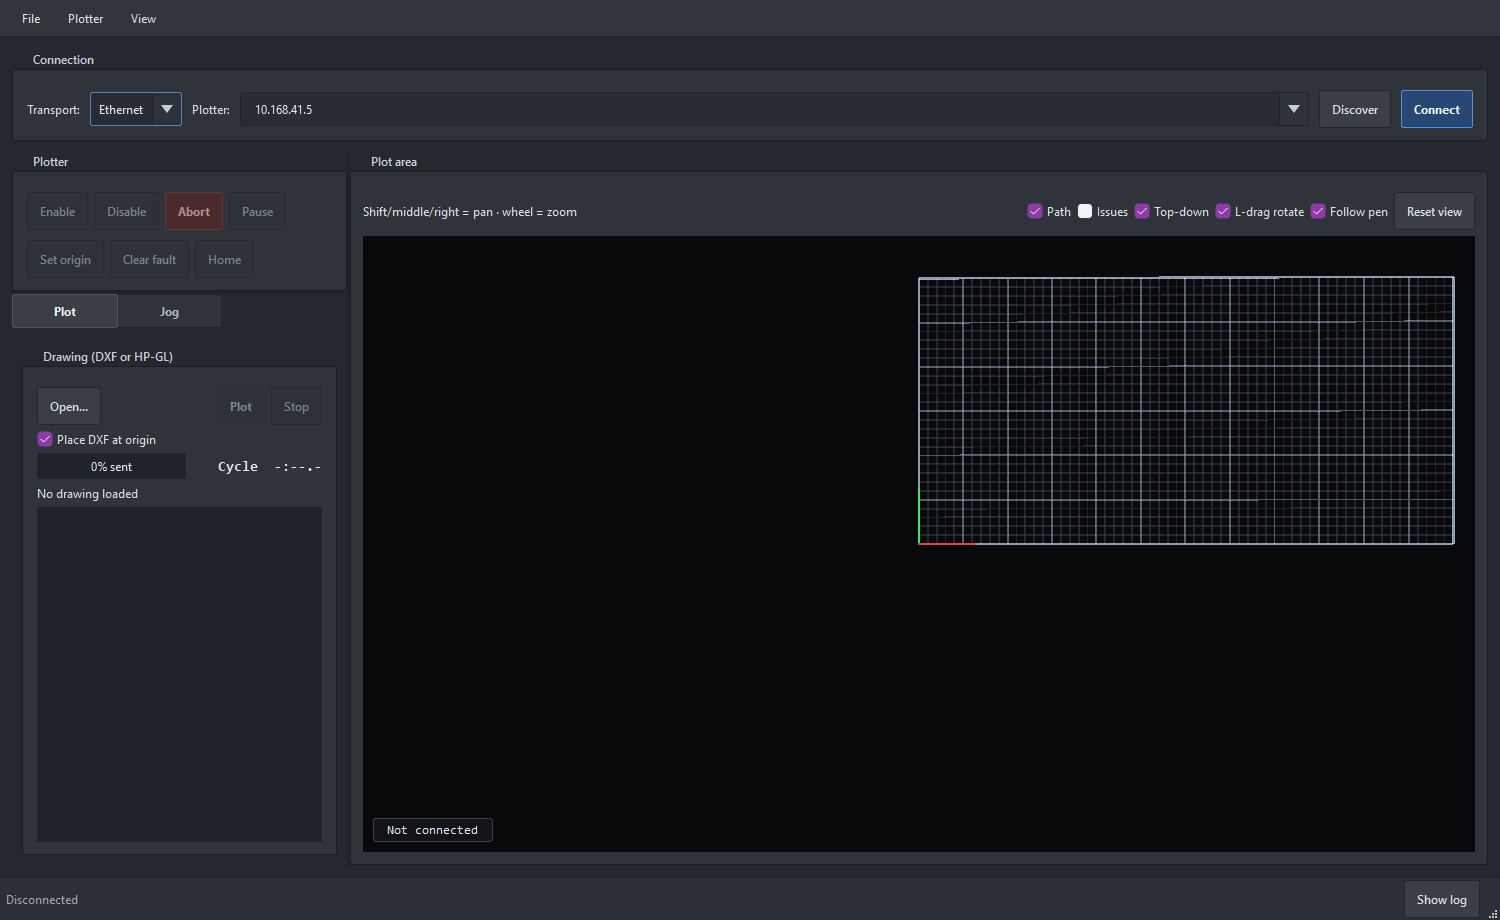
\includegraphics[width=\linewidth]{main-window.png}
\caption{The main window of the ClearHPGL app, before a connection}\label{fig:main}
\end{figure}

\section{Connect to the Plotter}

The app connects over Ethernet or over a serial port.

\begin{procedure}{Connect over Ethernet}
\begin{enumerate}
  \item Set \menu{Transport} to \menu{Ethernet}.
  \item Click \menu{Discover}. The app finds the boards on the local network
        and adds them to the \menu{Plotter} list.
  \item If the board is not found, type its IP address in \menu{Plotter}.
  \item Click \menu{Connect}.
\end{enumerate}
\end{procedure}

Over Ethernet, the app uses the console port (TCP 9300) for commands and
status, and the HP-GL port (TCP 9100) for jobs. The console port accepts one
client. While the app is connected, a terminal cannot use port 9300.

\begin{procedure}{Connect over a serial port}
\begin{enumerate}
  \item Set \menu{Transport} to \menu{Serial}.
  \item Click \menu{Refresh}, then select the COM port of the board.
  \item For the USB port, keep any baud rate and \menu{No flow control}.
  \item For \conn{COM-0} or \conn{COM-1}, set the baud rate to \key{com_baud}
        and the flow control to \key{com_handshake}.
  \item Click \menu{Connect}.
\end{enumerate}
\end{procedure}

When the app is connected, the status bar shows the state of the machine
(for example \code{idle}, \code{plotting}, or \code{fault}). The 3D view shows
the pen at its present position.

\section{Open a Drawing}

Click \menu{Open\ldots} on the \menu{Plot} tab, or use
\menu{File\,>\,Open drawing (DXF / HP-GL)\ldots}. The app opens two types of
file.

\subsection{HP-GL Files}

Files with the extension \file{.plt}, \file{.hpgl}, \file{.hgl}, \file{.hpg},
or \file{.prn}. The app sends the file to the board without changes. For the
preview, the app uses the HP-GL interpreter of the firmware. Thus the
position, the rotation, the scaling, and the clipping in the preview are the
same as on the machine.

\subsection{DXF Files}

The app reads ASCII DXF files. It reads these entities: \code{LINE},
\code{LWPOLYLINE}, \code{POLYLINE} (also with bulges), \code{ARC}, and
\code{CIRCLE}. It does not read binary DXF, text, splines, ellipses, or
blocks. In your CAD software, explode these objects into lines, arcs, and
polylines before you save the DXF.

\begin{caution}
The app uses the \code{\$INSUNITS} variable of the DXF to get the units. If
the DXF has no \code{\$INSUNITS}, or the value is 0 (unitless), the app uses
inches. Save the DXF with its units set, or the plot can be 25.4 times too
large or too small.
\end{caution}

The app prepares a DXF for plotting:

\begin{itemize}
  \item It joins lines whose ends touch into longer paths.
  \item It plots all shapes inside a closed contour before the contour.
        Thus holes are cut before the outline frees the part.
  \item It goes to the nearest shape next, to make the pen-up travel short.
  \item It sends arcs and circles as true arcs (HP-GL \cmd{AA}), not as
        short straight lines. The machine draws them as smooth curves.
\end{itemize}

When \menu{Place DXF at origin} is selected, the app moves the drawing so
that its lower-left corner is at plotter 0,0. Clear it to keep the
coordinates of the DXF.

\section{The 3D View}

The 3D view shows the bed as a grid with lines every \SI{10}{mm}. The drawing
is on the bed; pen-down lines and pen-up moves have different colors.

\begin{table}[htbp]
\centering
\caption{Controls of the 3D view}\label{tab:view}
\begin{tabularx}{\linewidth}{@{}P{0.3\linewidth}L@{}}
\toprule
\textbf{Control} & \textbf{Function} \\
\midrule
Mouse wheel & Zoom in and out. \\
Shift + drag, middle drag, or right drag & Move the view. \\
Left drag & Turn the view, when \menu{L-drag rotate} is selected. \\
\menu{Path} & Show or hide the drawing. \\
\menu{Issues} & Show or hide the markers for problems in the drawing. \\
\menu{Top-down} & Look straight down on the bed. \\
\menu{Follow pen} & Keep the pen in the center of the view while it plots. \\
\menu{Reset view} & Show the full drawing again. \\
\bottomrule
\end{tabularx}
\end{table}

\subsection{Problems in a Drawing}

When \menu{Issues} is selected, the view shows markers where the drawing can
give a bad result. Put the mouse on a marker to read the explanation. The app
finds these problems:

\begin{itemize}
  \item Contours that do not close (open profiles).
  \item Contours that almost touch across a pen-up move.
  \item Long pen-down jumps inside a path, and short gaps between long cuts.
  \item Corners so tight that the machine must slow down a lot.
  \item Lines that overlap or cross.
\end{itemize}

Right-click a marker for its menu. \menu{Copy explanation} and
\menu{Copy X, Y} copy the information. For a DXF, two quick fixes are
available:

\begin{description}[style=nextline,leftmargin=1.2em,font=\sffamily\bfseries\color{navy}]
  \item[Quick fix: close contour] Closes an open contour with a smooth bridge
        across the gap.
  \item[Quick fix: connect across pen-up] Joins two contours that almost touch
        into one path.
\end{description}

After a quick fix, the app orders the drawing again. Use
\menu{File\,>\,Save DXF geometry\ldots} to keep the repaired geometry in a
new DXF.

\section{Plot}

\begin{warning}
The machine moves when you click \menu{Plot}. Keep your hands out of the work
area.
\end{warning}

\begin{procedure}{Plot a drawing from the app}
\begin{enumerate}
  \item Connect to the plotter.
  \item Open the drawing.
  \item Look at the preview. Make sure that the drawing is in the plot area.
  \item Put the material and the pen on the machine.
  \item Click \menu{Plot}.
\end{enumerate}
\end{procedure}

Before the app sends a DXF job, it compares the drawing with the plot area of
the board. If shapes are outside the area, the app shows how many, and asks
you to continue or to stop. If the emergency stop input is open, the app does
not send the job.

During the plot:

\begin{itemize}
  \item The progress bar shows how much of the job the app has sent.
  \item The 3D view shows the pen, and paints the lines that are drawn in green.
  \item The HP-GL text below the progress bar highlights the instruction that
        the machine draws now.
  \item \menu{Cycle} shows the time from \menu{Plot} to the end of the plot.
\end{itemize}

The app also follows jobs from other programs. For example, when AutoCAD
plots on the USB port, the 3D view shows the pen and the lines that it draws.

\subsection{Pause and Stop}

\begin{description}[style=nextline,leftmargin=1.2em,font=\sffamily\bfseries\color{navy}]
  \item[Pause] The machine stops at the end of the segments in its queue and
        raises the pen. The button changes to \menu{Resume}. Click
        \menu{Resume} to lower the pen and continue.
  \item[Stop] The app stops sending and stops the plot on the board.
  \item[Abort] The board stops now, drops the job, and raises the pen. Use
        it for a job from any source.
\end{description}

\begin{warning}
\menu{Abort}, \menu{Stop}, and \menu{Pause} are not emergency stops. They
operate through the firmware and the link. Use the emergency stop if a person
or the machine is in danger.
\end{warning}

\section{Move the Pen}

The \menu{Jog} tab moves the pen with the pen up. The machine must not be
plotting.

\begin{itemize}
  \item \menu{Go to (pen up)}: type an X and a Y position in mm, then click
        \menu{Go}.
  \item \menu{Jog}: set \menu{Step (mm)}, then click \menu{X-}, \menu{X+},
        \menu{Y-}, or \menu{Y+}. The pen does not move out of the plot area.
  \item \menu{Pen up} and \menu{Pen down}: test the pen lift.
\end{itemize}

To make the present position the origin, click \menu{Set origin}.

\section{Plotter Settings}\label{sec:app-settings}

Use \menu{Plotter\,>\,Plotter settings\ldots} to change the settings of the
board. The app reads the settings from the board and shows them in groups
(figure~\ref{fig:settings}). Fixed choices are lists.

\begin{figure}[p]
\centering
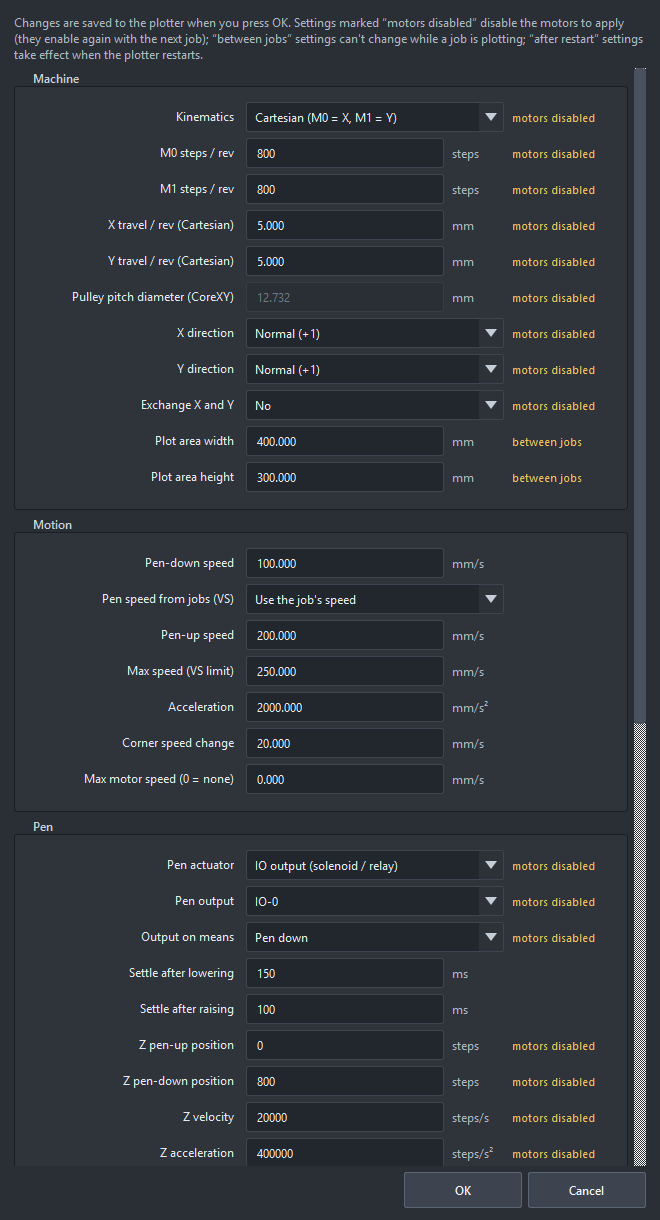
\includegraphics[width=0.78\linewidth]{settings-dialog.png}
\caption{The \menu{Plotter settings} dialog, with the factory settings}\label{fig:settings}
\end{figure}

A label next to a field tells you when the setting can change
(table~\ref{tab:when}):

\begin{description}[style=nextline,leftmargin=1.2em,font=\sffamily\bfseries\color{navy}]
  \item[motors disabled] The app disables the motors before it applies the
        change. The motors enable again with the next job.
  \item[between jobs] The change is not possible while a job plots, but the
        motors can stay enabled. The plot area has this label.
  \item[after restart] The board saves the change. It takes effect after the
        board restarts.
\end{description}

Click \menu{OK} to send the changes. The app does not send changes while a job
plots. If the board refuses a change, the app shows the settings that did not
change and the reason. The plot area of the app changes to the plot area of
the board.

\section{ClearPath Scope}\label{sec:scope}

\menu{Plotter\,>\,ClearPath scope\ldots} (Ctrl+Shift+O) records the signals
of the ClearPath servos through the USB port of each servo, the port that
ClearPath MSP uses. It shows them in lanes on one time axis
(figure~\ref{fig:scope}). Use it to see how the X and Y servos follow a plot:
the tracking error on each acceleration, the speed, the bus voltage, the
temperature, and the HLFB, enable, and alert signals.

The scope does not use the ClearCore. Thus it operates during a plot, and
over any link.

\begin{figure}[htbp]
\centering
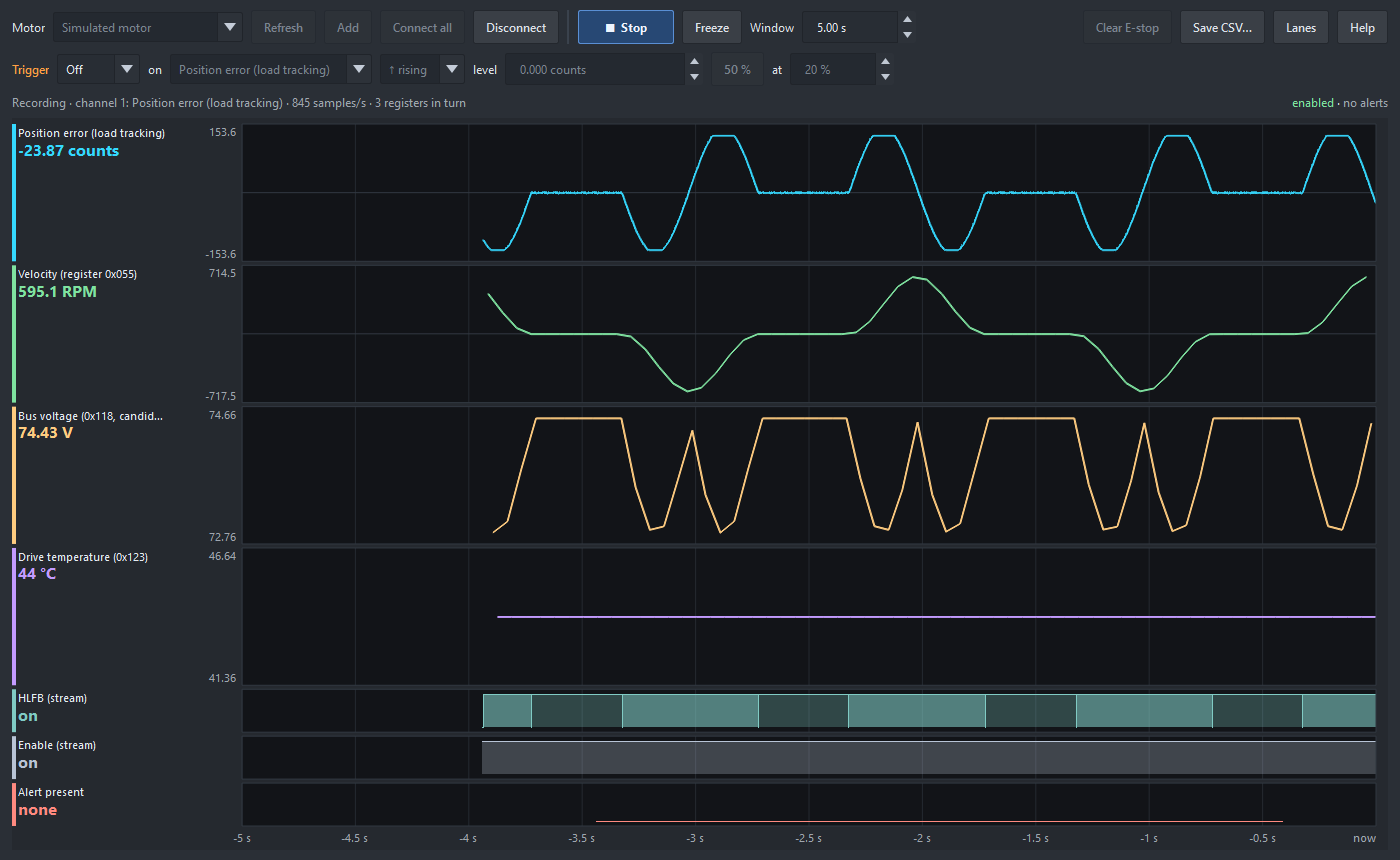
\includegraphics[width=\linewidth]{clearpath-scope.png}
\caption{The ClearPath scope, on its simulated motor}\label{fig:scope}
\end{figure}

\begin{procedure}{Record a ClearPath servo}
\begin{enumerate}
  \item Connect the USB port of the servo to the computer.
  \item Close ClearPath MSP. One program at a time can use the port.
  \item Select \menu{Plotter\,>\,ClearPath scope\ldots}.
  \item In \menu{Motor}, select the servo (\emph{ClearPath on COMn}). For more
        than one servo, click \menu{Connect all}.
  \item Click \menu{Connect}, then \menu{Start}.
  \item Click \menu{Stop} to stop the recording, then \menu{Disconnect}.
\end{enumerate}
\end{procedure}

\begin{itemize}
  \item \menu{Lanes} selects the signals, their sequence, color, and scale.
  \item \menu{Trigger} holds the screen on a repeated event, for example
        HLFB going low at the start of each move.
  \item \menu{Freeze} holds the view while the recording continues.
        \menu{Save CSV\ldots} saves the recording.
  \item \menu{Help} (F1) opens the full description of the scope.
  \item Without a servo, select \menu{Simulated motor} to try the scope.
\end{itemize}

\begin{note}
\notelabel The scope sets the working monitor channel of the servo while it
records, and sets it back when it stops. It saves nothing in the servo, and
it never enables or moves the motor.
\end{note}

\section{Other Functions}

\begin{itemize}
  \item \menu{File\,>\,Export HP-GL\ldots} saves the job as an HP-GL file. For a
        DXF, it is the HP-GL that the app sends.
  \item \menu{View\,>\,Command log} shows all commands and replies.
  \item \menu{View\,>\,Clear pen trace} removes the green trace of the last plot.
\end{itemize}
